\documentclass[12pt]{article}
\usepackage{amsmath, amssymb, amsthm, graphicx}

\title{APPM 4600 \\ Homework 2}
\author{Dani Lisle | STID:109 97 2839}
\date{\today}

\begin{document}
\maketitle

\section*{Problem 1}
\subsection*{Part a}

Given the binomial expansion,
\begin{equation*}
(1 + x)^n = 1 + n x + \frac{n(n-1)}{2!}x^2 + \ldots
\end{equation*}
As \(x \rightarrow 0\), the higher-order terms grow in total at a significantly lower rate then $x$, so we have
\begin{equation*}
(1 + x)^n = 1 + n x + o(x).
\end{equation*}

\newpage

\subsection*{Part b}

To show that $x \sin(\sqrt{x}) = O(x^{3/2})$ as $x \rightarrow 0$, we consider the function $f(x) = x \sin(\sqrt{x})$ and compare its growth rate to that of $g(x) = x^{3/2}$. We evaluate the derivatives of both functions:

\[
f'(x) = \frac{d}{dx}\left( x \sin(\sqrt{x}) \right) = \frac{\sqrt{x} \cos(\sqrt{x})}{2} + \sin(\sqrt{x})
\]

\[
g'(x) = \frac{d}{dx}\left( x^{3/2} \right) = 1.5x^{0.5}
\]

We then examine the limit of the ratio of these derivatives as $x$ approaches 0:

\[
\lim_{x \to 0} \frac{f'(x)}{g'(x)} = \lim_{x \to 0} \frac{\frac{\sqrt{x} \cos(\sqrt{x})}{2} + \sin(\sqrt{x})}{1.5x^{0.5}}
\]

Evaluating this limit yields:

\[
\lim_{x \to 0} \frac{f'(x)}{g'(x)} = 1
\]

This result indicates that the growth rate of $f(x)$ is comparable to that of $g(x)$ as $x$ approaches 0. Additionally, $f$'s growth slows as $x$ increases close to $0$, so $x \sin(\sqrt{x}) = O(x^{3/2})$ as $x \rightarrow 0$.

\subsection*{Part c}

To show that \(e^{-t} = o\left(\frac{1}{t^2}\right)\) as \(t \rightarrow \infty\), we evaluate the limit of the ratio of \(e^{-t}\) to \(\frac{1}{t^2}\) as \(t\) approaches infinity:

\[
\lim_{t \to \infty} \frac{e^{-t}}{\frac{1}{t^2}} =  \lim_{t \to \infty} \frac{t^2}{e^t} = \lim_{t \to \infty} \frac{t^2}{e^t} = \lim_{t \to \infty} \frac{2}{e^t} = 0
\]

After repeated applications of L'Hopital's Rule, the exponential term \(e^{-t}\) in the numerator ensures that the limit approaches 0, as the exponential decay outpaces any polynomial decay, satisfying the condition for \(e^{-t} = o\left(\frac{1}{t^2}\right)\).


\subsection*{Part d}

The integral is bounded by a constant multiple of $\epsilon$: $k \epsilon$ which is greater than or equal to the largest slice of the integral (which is that closest to zero). Therefore, the integral is $O(\epsilon)$.
Bounded by a constant multiple of $\epsilon$.

\newpage

\section*{Problem 2}

\subsection*{Part a}

The change in the solution $\Delta x$ due to the perturbation in $b$ can be calculated using the formula $\Delta x = A^{-1} \Delta b$:

\[
\Delta x = 
\begin{bmatrix}
1 - 10^{10} & 10^{10} \\
-10^{10} & 1 + 10^{10}
\end{bmatrix}
\begin{bmatrix}
\Delta b_1 \\
\Delta b_2
\end{bmatrix}
=
\begin{bmatrix}
-(10^{10} - 1)\Delta b_1 + 10^{10}\Delta b_2 \\
-10^{10}\Delta b_1 + (10^{10} + 1)\Delta b_2
\end{bmatrix}
\]

\subsection*{Part b}

The norm of A is 1, and the norm of A inverse is $2 \cdot 10^10$. See norm.py in the Homework 2 folder of the Git repository.

So the condition number is $1 \cdot 2 \cdot 10^{10} = 2 \cdot 10^{10}$.

\section*{Part c}

The error in the solution is bounded above by $2 \cdot 10^{10} * P_r$, where $P_r$ is the relative perturbation $\frac{||\Delta b||}{||b||}$. 


If $ \Delta b = \begin{bmatrix} p \times 10^{-5} \\ q \times 10^{-5} \end{bmatrix} $ then the upper bound is 

$$2 \cdot 10^{10} \cdot \sqrt{(p^2 + q^2)} \cdot 10^{-5} = 2\sqrt{(p^2 + q^2)} \cdot 10^5$$

With the Euclidean norm, the behavior is not qualitatively different when the perturbations are the same. Given both components have same true value, equal perturbations are more likely.

\newpage

\section*{Problem 3}

\subsection*{Part a}

Given the function \( f(x) = e^x - 1 \), the relative error can be bounded by the function's condition number \( k_f(x) \):

\[
\frac{|f(x) - \tilde{f}(x)|}{|f(x)|} \leq k_{f}(x) \frac{|x - \tilde{x}|}{|x|}
\]

where the condition number \( k_f(x) \) is defined as:

\[
k_{f}(x) = \left| \frac{x f'(x)}{f(x)} \right|
\]

For the given function \( f(x) = e^x - 1 \), the condition number becomes:

\[
k_{f}(x) = \left| \frac{x e^x}{e^x - 1} \right|
\]

Evaluating the limit as \( x \) approaches 0:

\[
\lim_{x \to 0} \frac{x e^x}{e^x - 1} = \lim_{x \to 0} \frac{e^x + x e^x}{e^x} = \lim_{x \to 0} (1 + x) = 1
\]

\subsection*{Part b}

When \( x \) is very large:

\[
\lim_{x \to \infty} \frac{x e^x}{e^x - 1} = \lim_{x \to \infty} (1 + x) = \infty
\]

This indicates that the algorithm is stable due to the condition number when \( x \) is not large.

\subsection*{Part c}

The algorithm gives 8 correct digits, this is expected because the error is on the same order of magnitude as the relative error for \( x \) and \( f(x) \).

\subsection*{Part d}

We seek a polynomial \( P_n \) such that:

\[
\frac{|f - \tilde{f}|}{|f|} \leq 10^{-16}
\]

The polynomial approximation \( P(x) \) is given by:

\[
P(x) = (e^{x_0} - 1) + (x - x_0)e^{x_0} + \frac{(x - x_0)^2 e^{x_0}}{2!} + \ldots
\]

The second-degree polynomial approximation \( P_2 \) is:

\[
P_2 = f(0) + f'(0) x
\]

\section*{Problem 4}

\section*{Part a}

Create vector $t$ from $0$ to $pi$ incrementing by $pi/30$, vector y equal to $\cos(1)$. Write code that evaluates the specified sum and prints the result.

\begin{verbatim}
	The sum is: -23.915381134014112
\end{verbatim}

See t\_y\_sum.py in Git repository. The code simply creates vectors with np.arane() and evaluates with np.sum().

The true value is -2 (as can be trivially found with a single application of IBP). 

The closest lowest error we can achieve using this algorithm requires us to to use a dt of pi/2. This error is due to cancellation from to the negative terms.

\newpage

\section*{Part b}

Plot a parametric curve for $x(\theta)$ with given parameters. Adjust the scale so that the axes have the same scale. In a second figure, plot 10 curves with varying parameters.

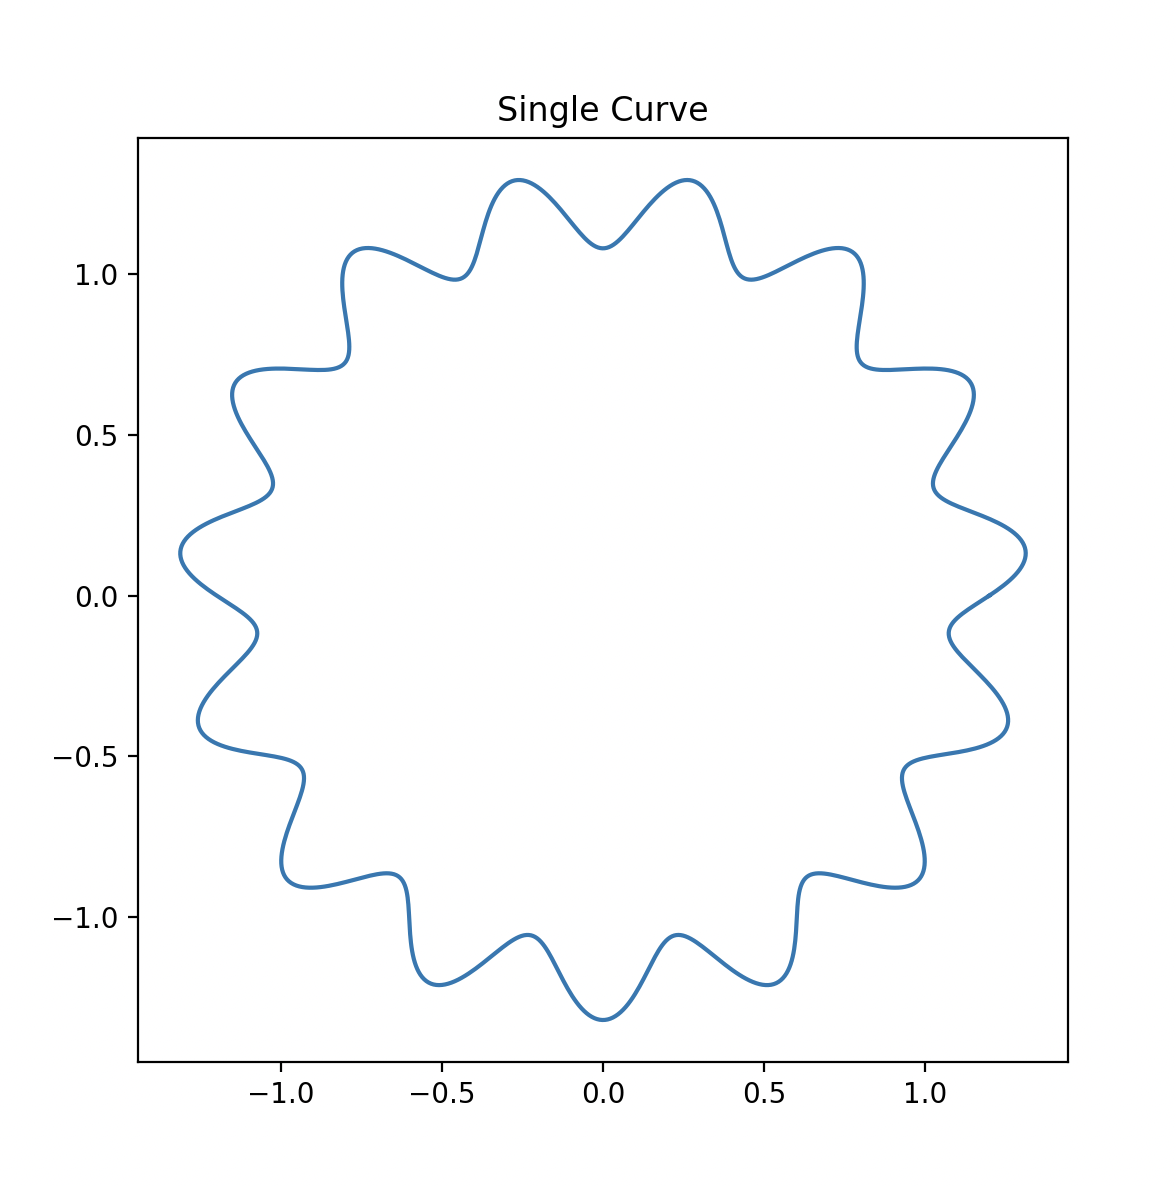
\includegraphics[width=0.5\textwidth]{screenshot2.png}


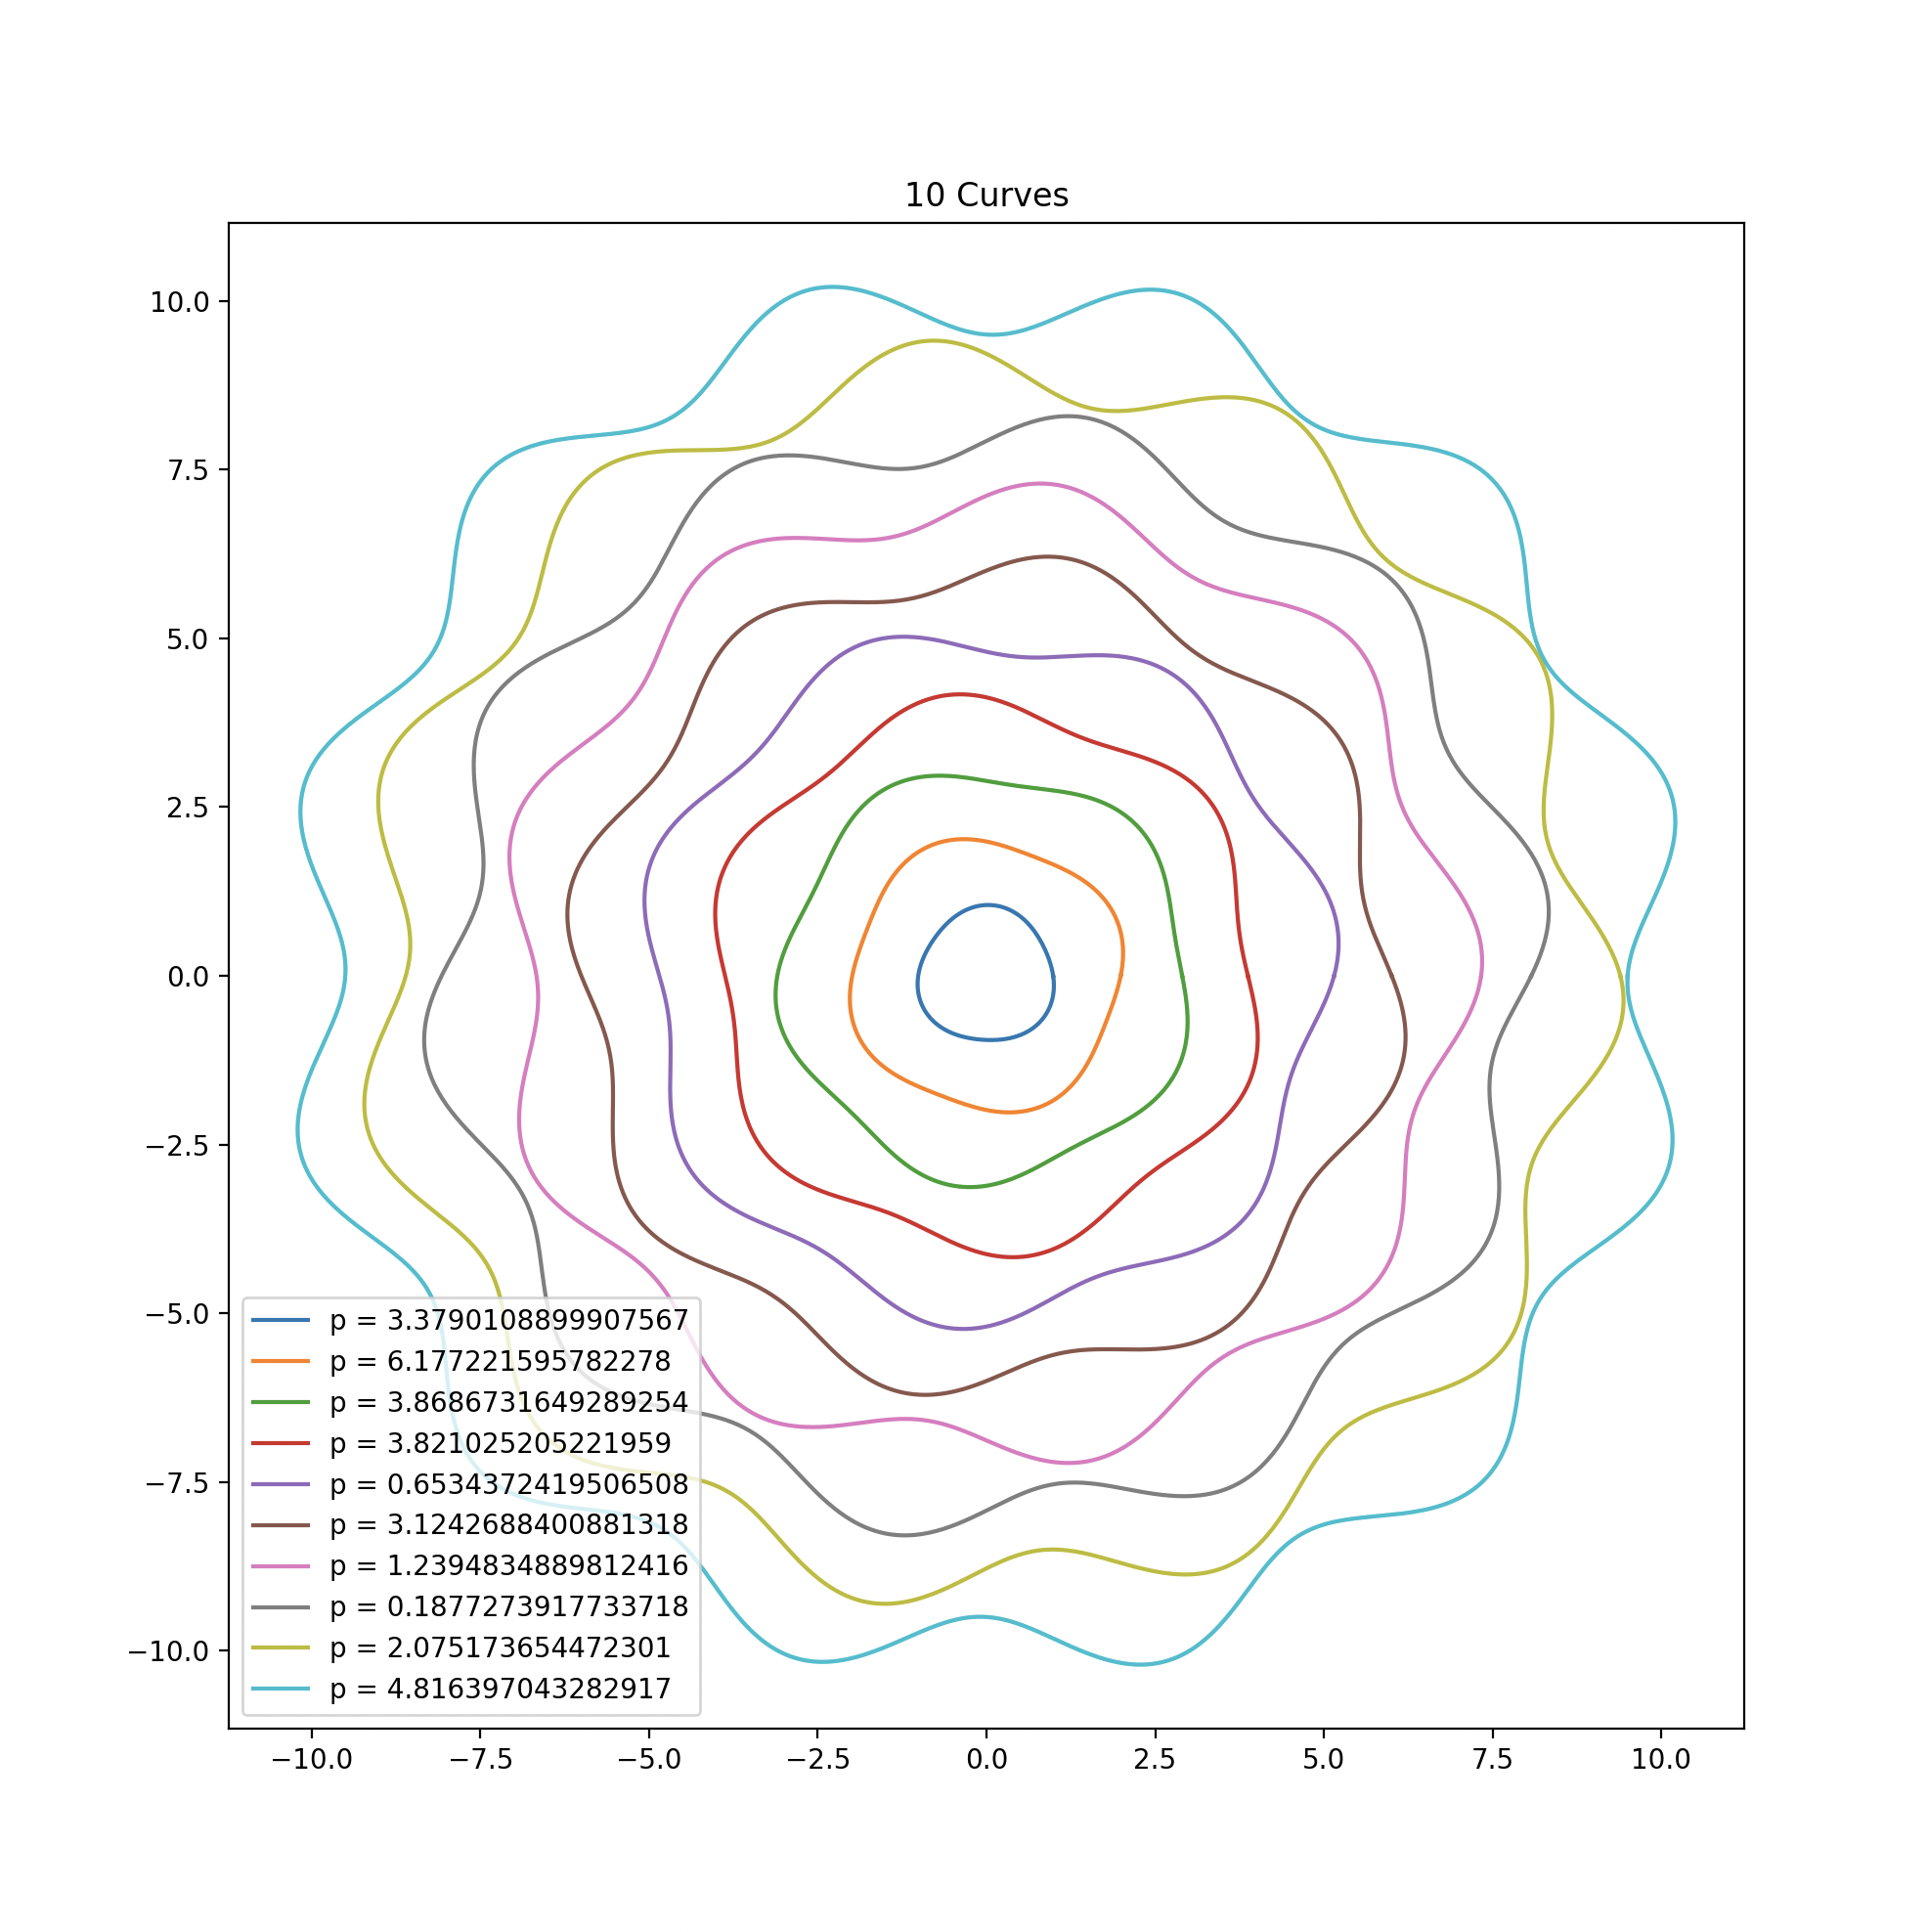
\includegraphics[width=0.5\textwidth]{screenshot1.png}

See wavy\_circles.py in Git repository.



\end{document}